Phần này trình bày các Sequence Diagrams mô tả luồng tương tác giữa các thành phần hệ thống (Frontend, Controllers, Services, Database) thông qua các lời gọi API, kiểm tra điều kiện và phản hồi theo từng module. Mỗi module có mô tả tổng quan và các diagram chi tiết với hình ảnh minh họa.

\subsection{Module 1 – Quản lý Người dùng và Xác thực}

Module này mô tả luồng tương tác trong xác thực người dùng: đăng ký, đăng nhập với 2FA, khôi phục mật khẩu, quản lý hồ sơ, và nâng cấp lên Seller. Các diagram thể hiện cách Frontend giao tiếp với AuthController, UserController, EmailService và TokenService.

\subsubsection{SD-M1-Auth-RegisterLogin}

Diagram này mô tả chuỗi tương tác trong quá trình đăng ký và đăng nhập, bao gồm ba use case chính.

\textbf{UC1.1 – Đăng ký tài khoản:} Frontend gửi POST \texttt{/api/auth/register} với dữ liệu đăng ký. AuthController kiểm tra email đã tồn tại trong DB chưa. Nếu đã tồn tại, trả về 409 (Conflict). Nếu hợp lệ, AuthController tạo tài khoản với trạng thái \textit{unverified} và vai trò \textit{buyer}, gọi EmailService gửi email xác thực, và trả về 201 (Created).

\textbf{UC1.2 – Đăng nhập:} Frontend gửi POST \texttt{/api/auth/login} với email và mật khẩu. AuthController xác thực thông tin trong DB. Nếu sai/khóa/chưa xác thực, trả về 401/403. Nếu đúng và không bật 2FA, AuthController gọi TokenService tạo JWT, trả về 200 kèm token. Nếu bật 2FA, chuyển sang UC1.3.

\textbf{UC1.3 – Xác thực hai yếu tố (2FA):} AuthController gọi EmailService gửi mã OTP. Người dùng nhập mã OTP, Frontend gửi POST \texttt{/api/auth/verify-2fa}. AuthController kiểm tra mã OTP trong DB. Nếu hợp lệ, tạo JWT và trả về 200. Nếu sai/hết hạn, trả về 401.

\begin{figure}[H]
  \centering
  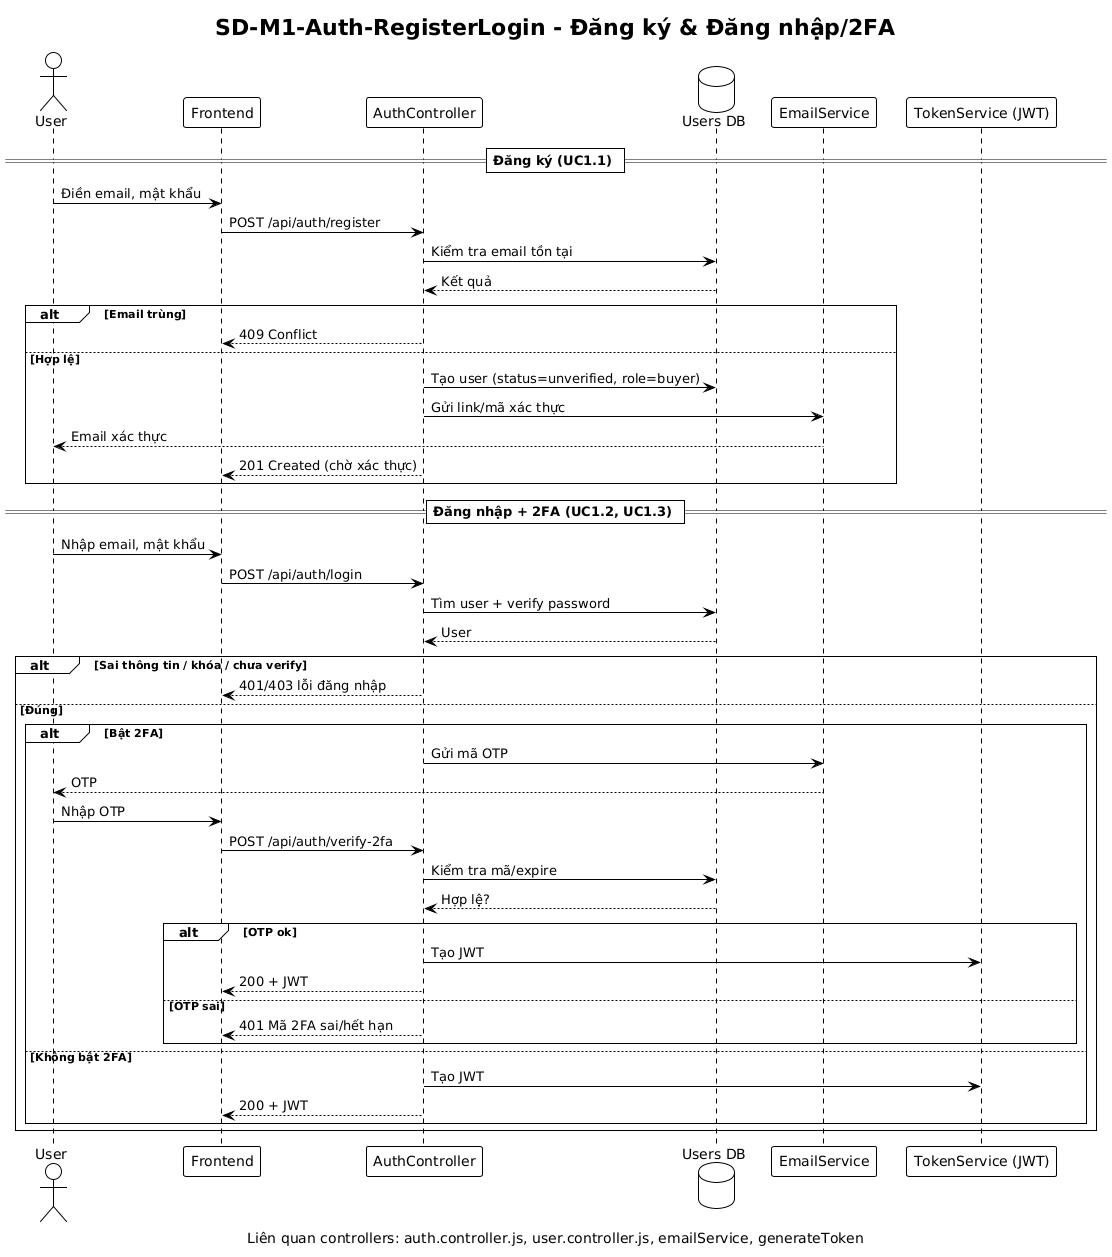
\includegraphics[width=\textwidth]{Images/Sequence diagrams/SD-M1-Auth-RegisterLogin.png}
  \caption{Sequence Diagram - Đăng ký và Đăng nhập (SD-M1-Auth-RegisterLogin)}
\end{figure}

\subsubsection{SD-M1-Auth-RecoveryLogout}

Diagram này mô tả chuỗi tương tác trong quá trình khôi phục mật khẩu và đăng xuất.

\textbf{UC1.4 – Khôi phục mật khẩu:} Frontend gửi POST \texttt{/api/auth/forgot-password} với email. AuthController xử lý yêu cầu theo cơ chế trả thông báo chung để tránh lộ thông tin tài khoản. Nếu email tồn tại, hệ thống tạo token reset, lưu vào DB và gọi EmailService gửi email. Người dùng mở link và đặt mật khẩu mới. Frontend gửi POST \texttt{/api/auth/reset-password} với token và mật khẩu mới. AuthController xác thực, hash mật khẩu và cập nhật trong DB, trả về 200.

\textbf{UC1.5 – Đăng xuất:} Frontend gửi POST \texttt{/api/auth/logout}. AuthController trả về kết quả đăng xuất, sau đó Frontend xóa token khỏi local storage và chuyển hướng về Trang chủ.

\begin{figure}[H]
  \centering
  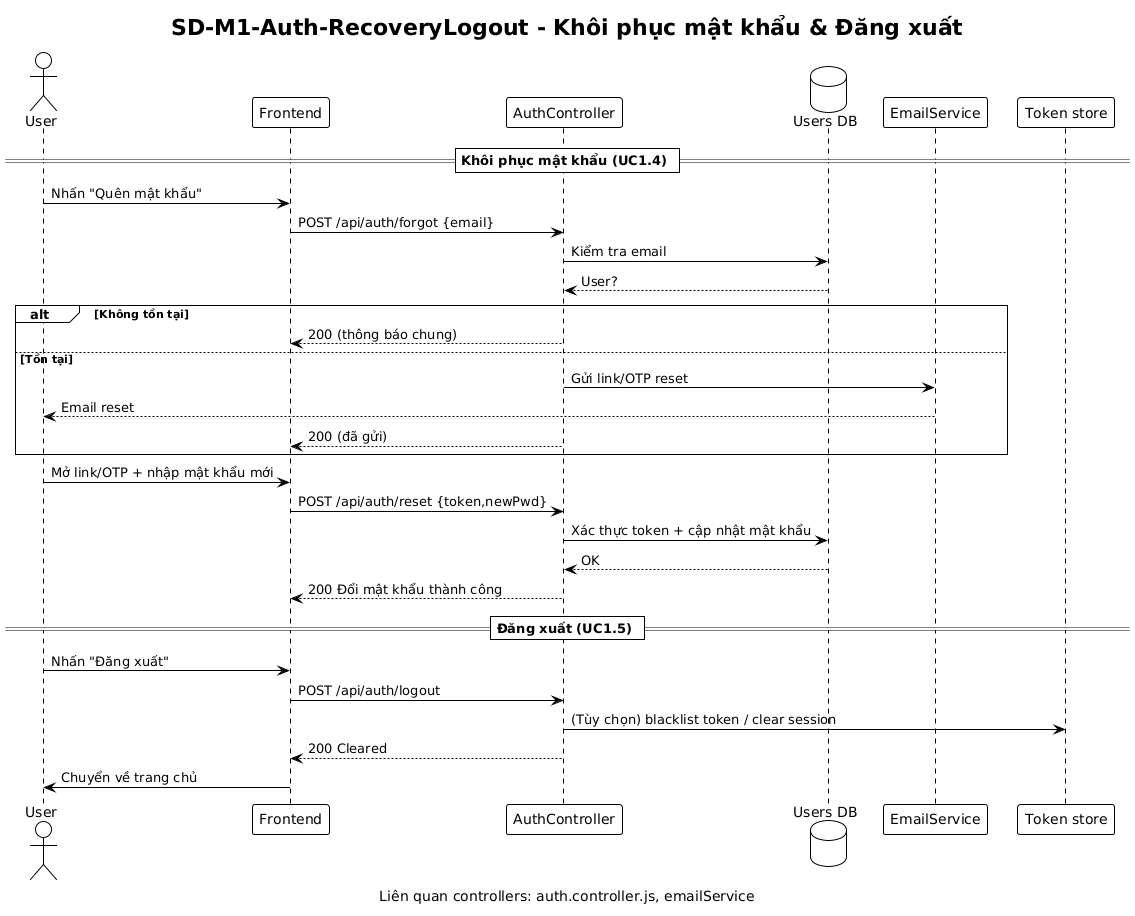
\includegraphics[width=\textwidth]{Images/Sequence diagrams/SD-M1-Auth-RecoveryLogout.png}
  \caption{Sequence Diagram - Khôi phục mật khẩu và Đăng xuất (SD-M1-Auth-RecoveryLogout)}
\end{figure}

\subsubsection{SD-M1-Profile-EditPrivacy}

Diagram này mô tả chuỗi tương tác trong quá trình chỉnh sửa hồ sơ và cài đặt quyền riêng tư.

\textbf{UC1.6 – Chỉnh sửa hồ sơ:} Frontend gửi PUT \texttt{/api/users/me} kèm dữ liệu cập nhật, file ảnh (nếu có) và JWT token. UserController xác thực token, nếu có ảnh thì gọi Storage service upload và nhận URL ảnh. UserController cập nhật thông tin trong Users DB, trả về 200 kèm hồ sơ mới.

\textbf{UC1.7 – Quyền riêng tư:} Frontend gửi PUT \texttt{/api/auth/privacy} kèm cấu hình quyền riêng tư và JWT token. AuthController xác thực token, lưu cấu hình vào Users DB và trả về 200.

\begin{figure}[H]
  \centering
  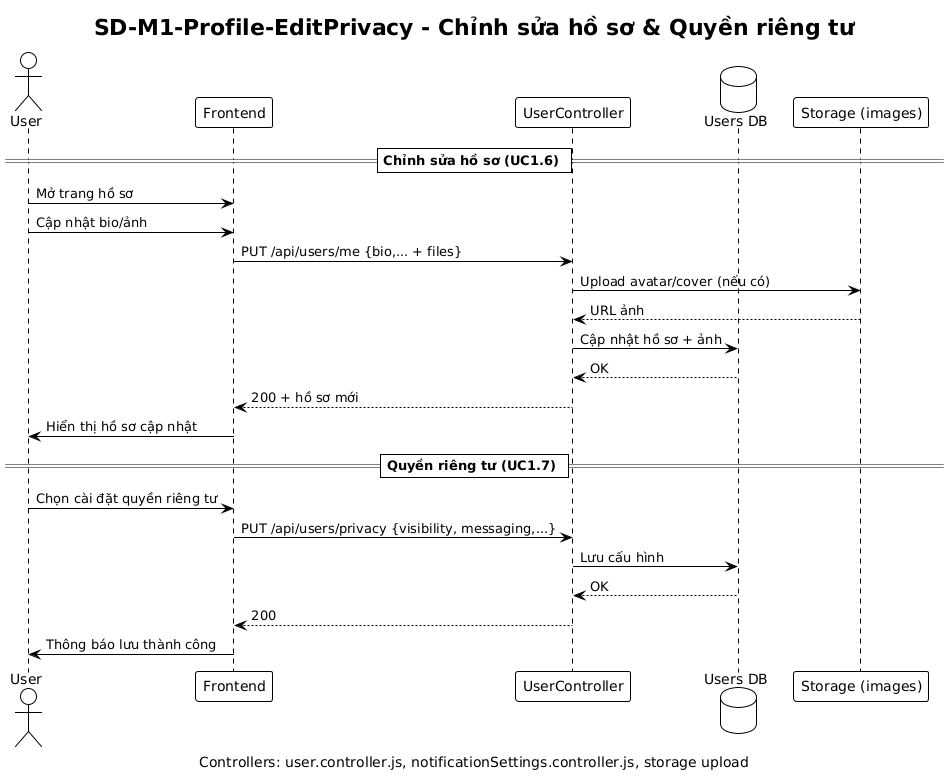
\includegraphics[width=\textwidth]{Images/Sequence diagrams/SD-M1-Profile-EditPrivacy.png}
  \caption{Sequence Diagram - Chỉnh sửa hồ sơ và Quyền riêng tư (SD-M1-Profile-EditPrivacy)}
\end{figure}

\subsubsection{SD-M1-Profile-SellerUpgrade}

Diagram này mô tả chuỗi tương tác trong quá trình đăng ký trở thành người bán.

\textbf{UC1.8 – Đăng ký Người bán:} Frontend gửi POST \texttt{/api/seller/apply} để khởi tạo hồ sơ, sau đó gửi dữ liệu qua các endpoint nhiều bước như \texttt{/api/seller/step1}, \texttt{/api/seller/step2}, \texttt{/api/seller/step3} hoặc \texttt{/api/seller/register-with-uploads}. SellerController xác thực, lưu hồ sơ vào bảng \textit{seller\_verifications} và chuyển trạng thái sang chờ duyệt. Admin xử lý qua admin API; nếu duyệt, hệ thống cập nhật role của user thành \textit{SELLER}.

\begin{figure}[H]
  \centering
  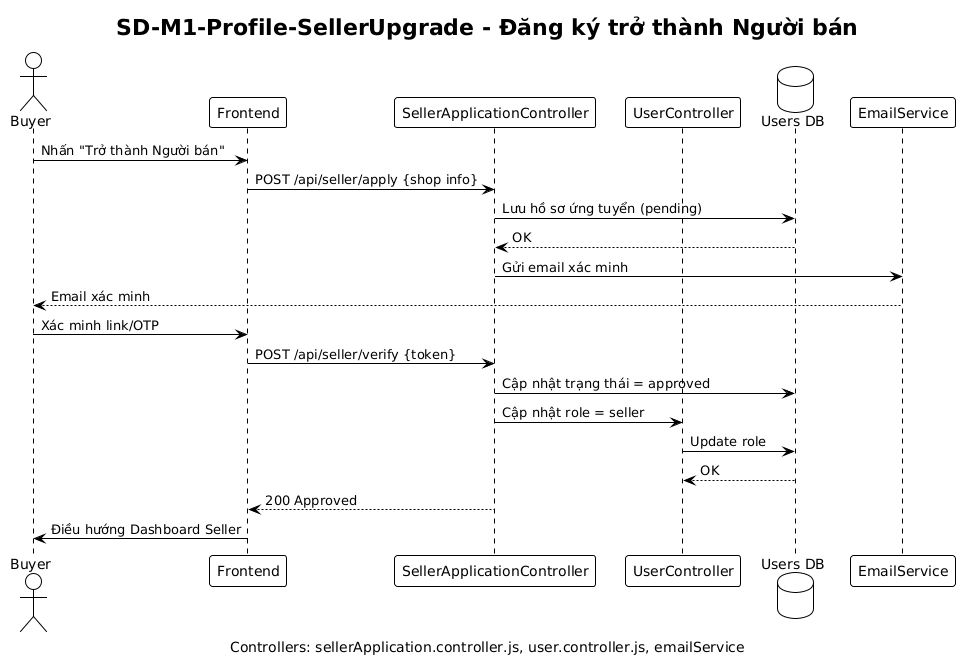
\includegraphics[width=\textwidth]{Images/Sequence diagrams/SD-M1-Profile-SellerUpgrade.png}
  \caption{Sequence Diagram - Đăng ký trở thành Người bán (SD-M1-Profile-SellerUpgrade)}
\end{figure}

\subsection{Module 2 – Tương tác Xã hội}

Module này mô tả luồng tương tác trong tính năng mạng xã hội: xem feed, tạo và tương tác với bài đăng, follow, nhắn tin, tham gia nhóm, báo cáo vi phạm. Các diagram thể hiện cách Frontend giao tiếp với PostController, UserController, MessageController, ReportController, FeedService, ProductController và NotificationService.

\subsubsection{SD-M2-FeedAndPosts}

Diagram này mô tả chuỗi tương tác trong quá trình xem feed, tạo bài đăng và tương tác với nội dung.

\textbf{UC2.1 – Xem Feed:} Frontend gửi GET \texttt{/api/posts/feed} kèm JWT token và tham số phân trang để lấy personalized feed, hoặc GET \texttt{/api/posts} cho feed công khai. PostController gọi PostService truy vấn DB lấy bài đăng từ người đang theo dõi kết hợp gợi ý, trả về danh sách đã sắp xếp. Frontend hiển thị với infinite scroll.

\textbf{UC2.2 và UC2.3 – Tạo bài đăng và gắn thẻ sản phẩm:} Nếu Seller muốn gắn sản phẩm, Frontend có thể lấy sản phẩm của seller qua các endpoint sản phẩm dành cho seller như \texttt{/api/products/seller/me}. Sau khi chọn một hoặc nhiều sản phẩm, Frontend gửi POST \texttt{/api/posts} kèm nội dung, media, mảng \texttt{productTags} và JWT token. PostController xác thực, kiểm tra nội dung, PostService lưu bài đăng vào \textit{posts} và lưu các tag vào \textit{post\_product\_tags}, sau đó trả về 201.

\textbf{UC2.4 – Tương tác với bài đăng:} Frontend gửi POST \texttt{/api/posts/:id/like} hoặc \texttt{/api/posts/:id/comments} kèm nội dung (nếu comment) và JWT token. PostController xác thực, lưu lượt thích/bình luận vào DB, gọi NotificationService gửi thông báo đến chủ sở hữu bài đăng, trả về 200 kèm trạng thái mới.

\begin{figure}[H]
  \centering
  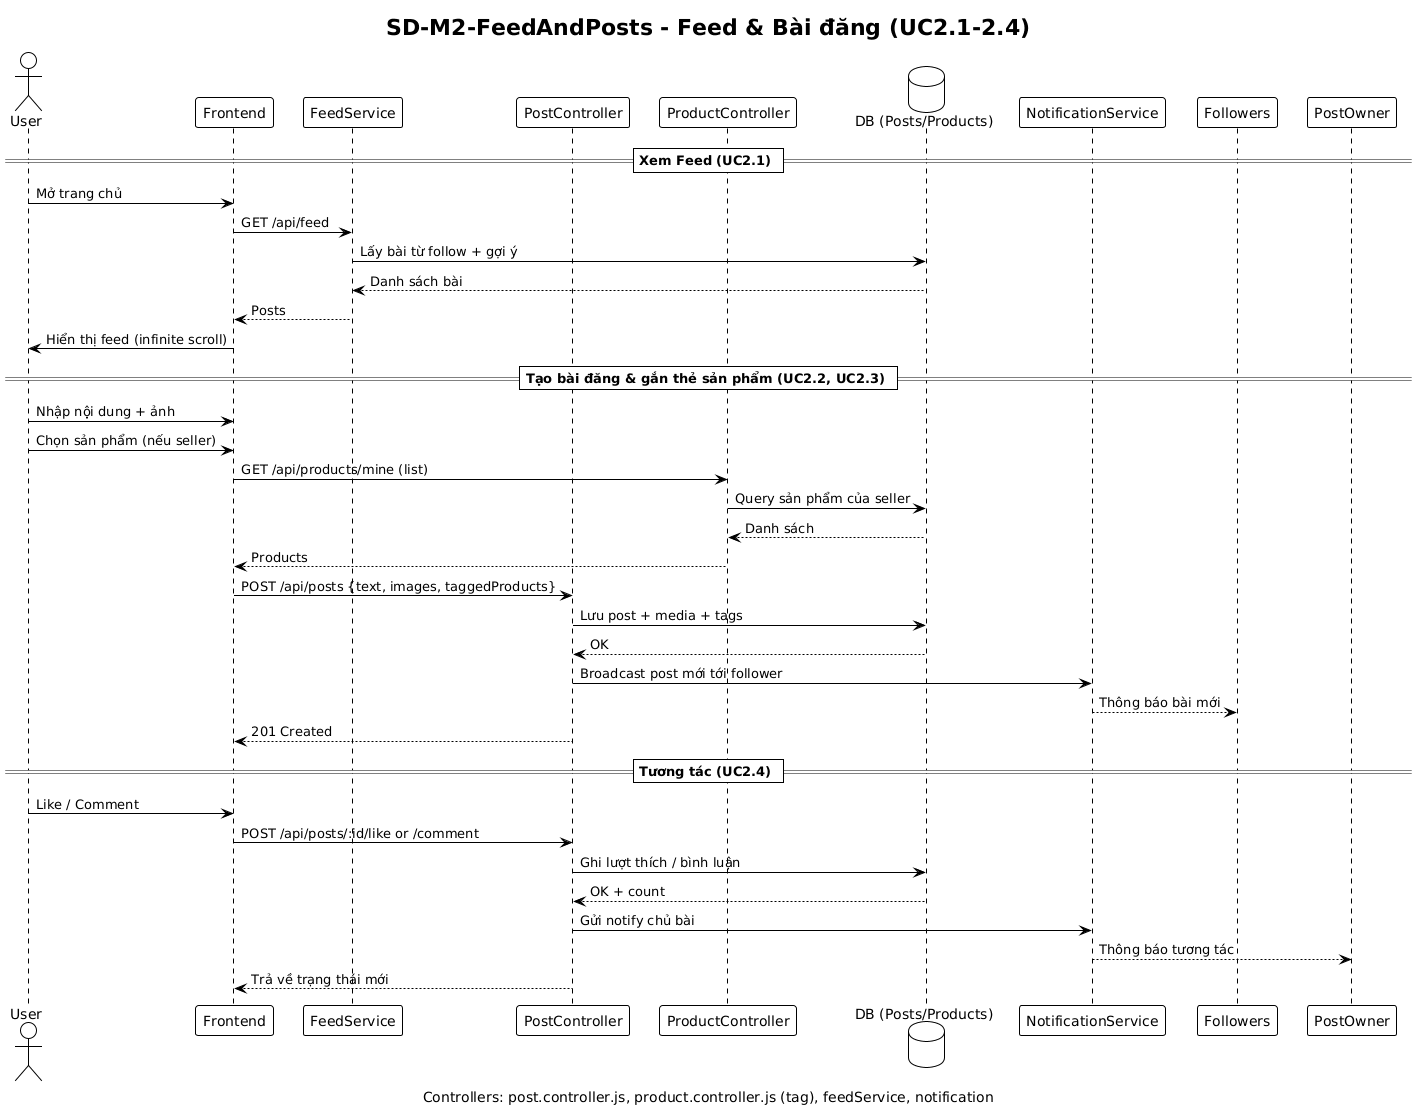
\includegraphics[width=\textwidth]{Images/Sequence diagrams/SD-M2-FeedAndPosts.png}
  \caption{Sequence Diagram - Feed và Bài đăng (SD-M2-FeedAndPosts)}
\end{figure}

\subsubsection{SD-M2-SocialConnections}

Diagram này mô tả chuỗi tương tác trong các kết nối xã hội giữa người dùng.

\textbf{UC2.5 – Theo dõi người dùng:} Frontend gửi POST \texttt{/api/users/:bId/follow} kèm JWT token. UserController xác thực, kiểm tra A chưa follow B, tạo mối quan hệ UserFollow trong DB, gọi NotificationService gửi thông báo đến B, trả về 200.

\textbf{UC2.6 – Nhắn tin 1-1:} Frontend gửi POST \texttt{/api/messages/conversations} để lấy hoặc tạo conversation với người nhận. Khi gửi tin nhắn, Frontend gửi POST \texttt{/api/messages/conversations/:conversationId} kèm nội dung và JWT token. MessageController xác thực người gửi thuộc conversation, lưu tin nhắn vào DB, emit realtime qua Socket.IO và tạo notification nếu người nhận offline.

\textbf{UC2.7 – Tham gia nhóm:} Frontend gửi POST \texttt{/api/groups/:groupId/join} kèm JWT token. GroupController xác thực, kiểm tra loại nhóm. Nếu công khai, thêm membership ngay; nếu riêng tư, tạo yêu cầu tham gia với trạng thái \textit{pending}. Lưu vào DB và trả về kết quả.

\textbf{UC2.8 – Báo cáo vi phạm:} Frontend gửi POST \texttt{/api/reports} kèm targetType, targetId, reason, description (nếu có) và JWT token. ReportController xác thực, lưu báo cáo với trạng thái \textit{pending} vào DB và trả về kết quả. Admin xem báo cáo qua admin API.

\begin{figure}[H]
  \centering
  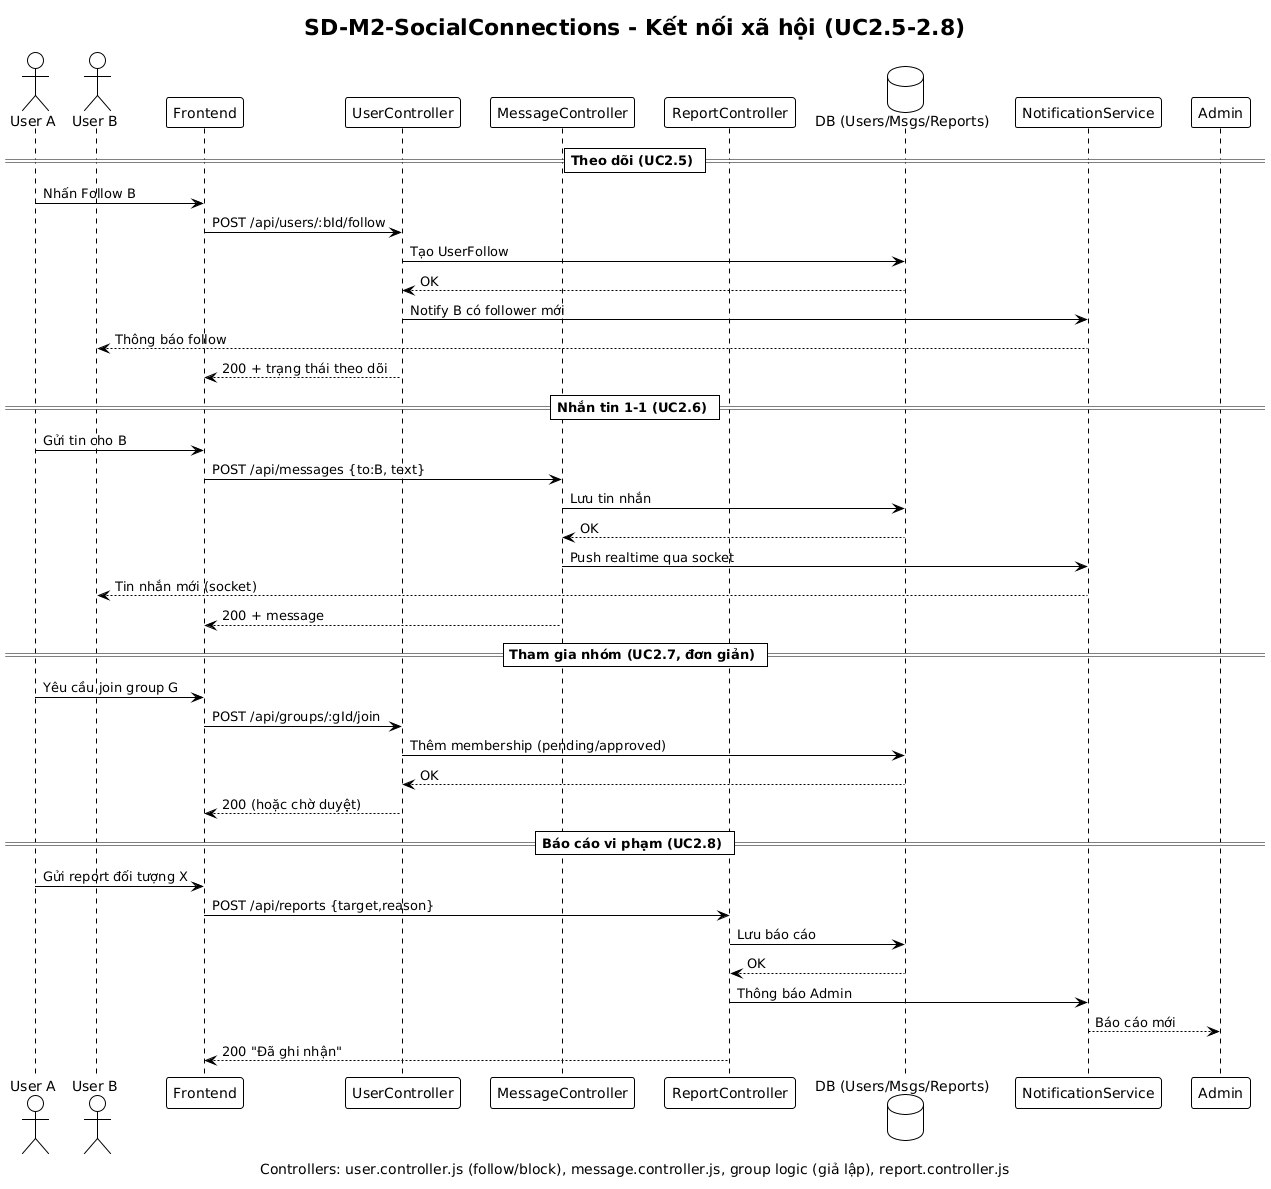
\includegraphics[width=\textwidth]{Images/Sequence diagrams/SD-M2-SocialConnections.png}
  \caption{Sequence Diagram - Kết nối Xã hội (SD-M2-SocialConnections)}
\end{figure}

\subsection{Module 3 – Hoạt động Thương mại}

Module này mô tả luồng tương tác trong hệ sinh thái thương mại: hành trình mua hàng của Buyer (tìm kiếm, xem sản phẩm, giỏ hàng, thanh toán, theo dõi đơn hàng, đánh giá) và tác vụ của Seller (quản lý sản phẩm, xử lý đơn hàng, hoàn tiền, phản hồi đánh giá). Các diagram thể hiện cách Frontend giao tiếp với ProductController, CartController, OrderController, ReviewController và NotificationService.

\subsubsection{SD-M3-BuyerFlow}

Diagram này mô tả chuỗi tương tác trong toàn bộ quy trình mua hàng từ góc nhìn của Buyer.

\textbf{UC3.1 và UC3.2 – Tìm kiếm và xem sản phẩm:} Frontend gửi GET \texttt{/api/products?query=...\&filters=...} với tham số tìm kiếm và lọc. ProductController truy vấn DB, trả về danh sách sản phẩm. Frontend hiển thị danh sách. Để xem chi tiết, Frontend gửi GET \texttt{/api/products/:id}. ProductController truy vấn DB lấy chi tiết và biến thể, trả về dữ liệu chi tiết.

\textbf{UC3.3 và UC3.4 – Quản lý giỏ hàng:} Frontend gửi POST \texttt{/api/cart/items} kèm ID sản phẩm, biến thể, số lượng và JWT token. CartController xác thực, kiểm tra tồn kho, lưu cart item vào DB, trả về giỏ hàng đã cập nhật. Để cập nhật/xóa: Frontend gửi PATCH \texttt{/api/cart/items/:id} hoặc DELETE. CartController cập nhật/xóa trong DB, tính lại tổng tiền, trả về giỏ hàng đã cập nhật.

\textbf{UC3.5 – Thanh toán:} Frontend gửi POST \texttt{/api/orders} kèm thông tin giỏ hàng, địa chỉ giao hàng, phương thức thanh toán và JWT token. OrderController xác thực, kiểm tra tồn kho. Nếu đủ hàng, tạo Order với trạng thái \textit{Processing} và OrderItems trong DB, gọi NotificationService gửi thông báo đến Seller, trả về 201. Nếu hết hàng, trả về 400.

\textbf{UC3.6 và UC3.7 – Theo dõi đơn hàng và đánh giá:} Frontend gửi GET \texttt{/api/orders/my/purchases} kèm JWT token. OrderController xác thực, truy vấn DB lấy danh sách đơn hàng của Buyer, trả về danh sách. Khi đơn hàng đã giao hoặc hoàn thành, Frontend gửi POST \texttt{/api/reviews} kèm ID order item, số sao, nhận xét, hình ảnh (nếu có) và JWT token. ReviewController xác thực, lưu đánh giá vào DB, trả về 201.

\begin{figure}[H]
  \centering
  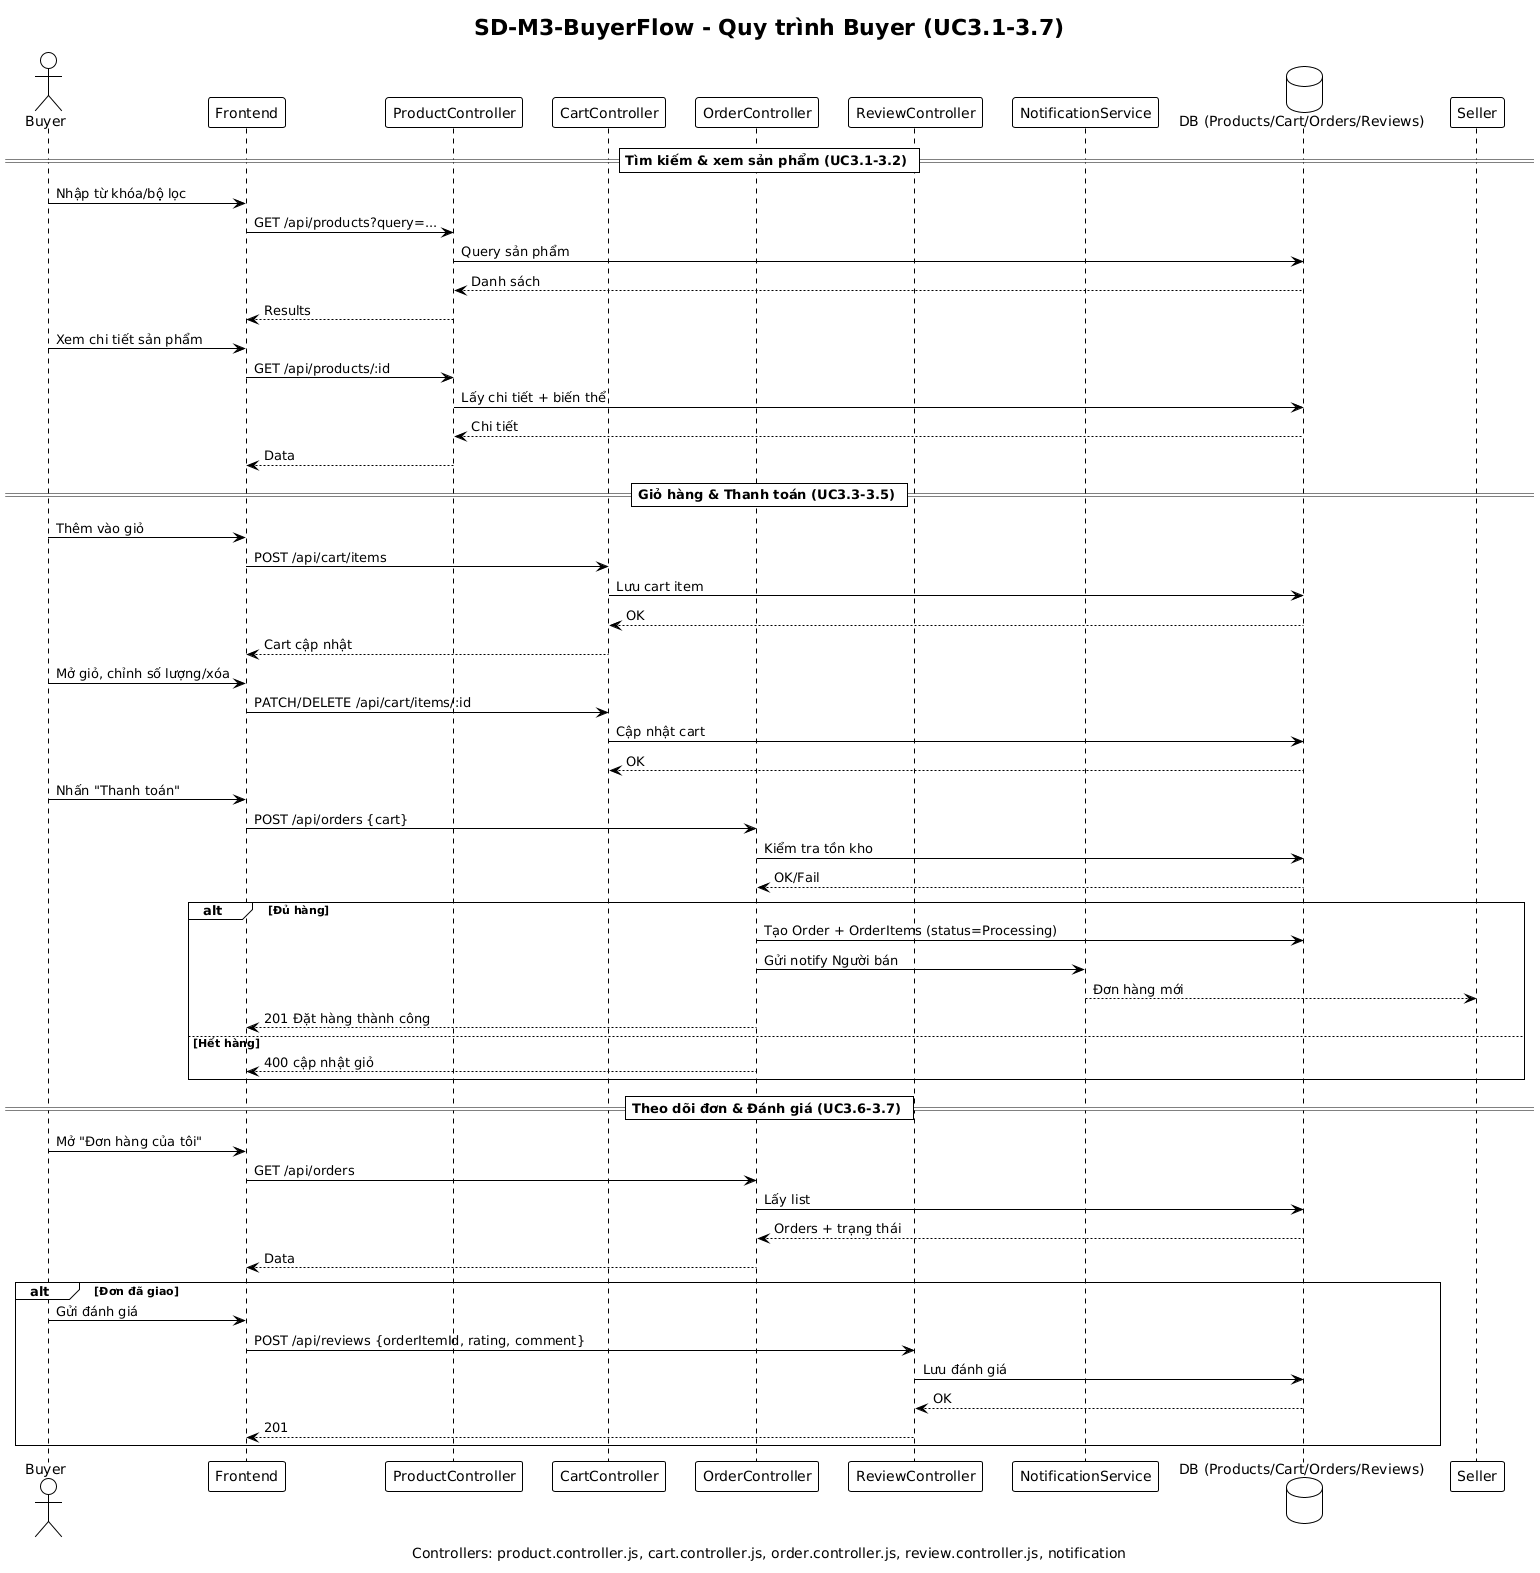
\includegraphics[width=\textwidth]{Images/Sequence diagrams/SD-M3-BuyerFlow.png}
  \caption{Sequence Diagram - Quy trình Mua hàng (SD-M3-BuyerFlow)}
\end{figure}

\subsubsection{SD-M3-Seller-ProductsOrders}

Diagram này mô tả chuỗi tương tác trong quá trình quản lý sản phẩm và đơn hàng của Seller.

\textbf{UC3.8 – Quản lý sản phẩm:} Frontend gửi POST \texttt{/api/products} (thêm), PUT \texttt{/api/products/:id} (sửa), hoặc DELETE \texttt{/api/products/:id} (xóa) kèm dữ liệu sản phẩm và JWT token. ProductController xác thực token và vai trò Seller, thực hiện lưu/cập nhật/soft-delete sản phẩm cùng biến thể trong DB, trả về 200/201.

\textbf{UC3.10 – Quản lý đơn hàng:} Frontend gửi GET \texttt{/api/orders/my/sales} kèm JWT token. OrderController xác thực token và vai trò Seller, truy vấn DB lấy danh sách đơn hàng của shop, trả về danh sách. Để cập nhật trạng thái: Frontend gửi PUT \texttt{/api/orders/:orderId/status} kèm trạng thái mới và JWT token. OrderController xác thực quyền, cập nhật trạng thái trong DB, gọi NotificationService thông báo Buyer, trả về 200.

\begin{figure}[H]
  \centering
  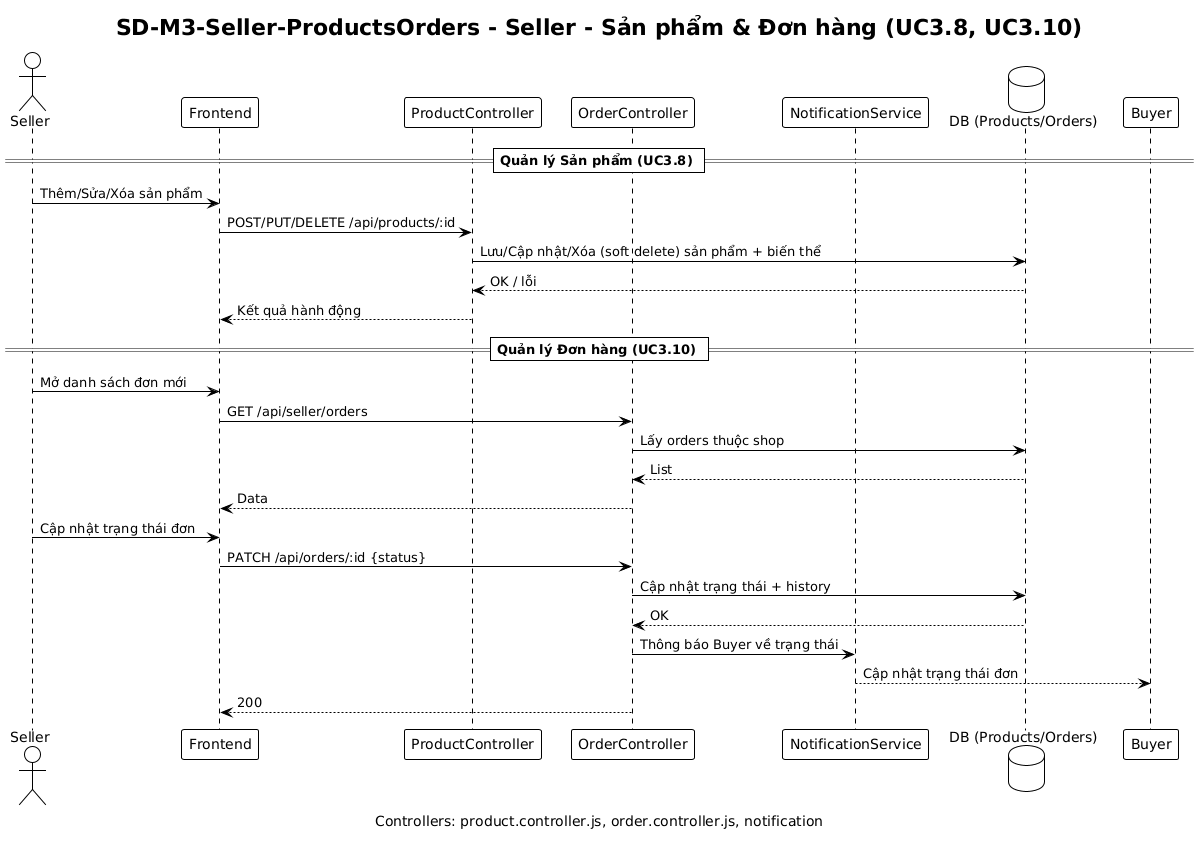
\includegraphics[width=\textwidth]{Images/Sequence diagrams/SD-M3-Seller-ProductsOrders.png}
  \caption{Sequence Diagram - Quản lý Sản phẩm và Đơn hàng của Seller (SD-M3-Seller-ProductsOrders)}
\end{figure}

\subsubsection{SD-M3-Seller-RefundReview}

Diagram này mô tả chuỗi tương tác trong quá trình xử lý hoàn tiền và phản hồi đánh giá của Seller.

\textbf{UC3.11 – Xử lý hoàn tiền:} Frontend gửi GET \texttt{/api/orders/seller/refunds} kèm JWT token. OrderController xác thực, truy vấn DB lấy danh sách yêu cầu hoàn tiền, trả về danh sách. Seller quyết định: Frontend gửi POST \texttt{/api/orders/:orderId/refund} kèm quyết định và lý do. OrderController cập nhật trạng thái/lý do liên quan trong phạm vi giả lập, gọi NotificationService thông báo Buyer và trả về kết quả.

\textbf{UC3.12 – Phản hồi đánh giá:} Frontend gửi POST \texttt{/api/reviews/:id/reply} kèm nội dung phản hồi và JWT token. ReviewController xác thực token và vai trò Seller, lưu phản hồi vào DB, gọi NotificationService thông báo Buyer, trả về 201.

\begin{figure}[H]
  \centering
  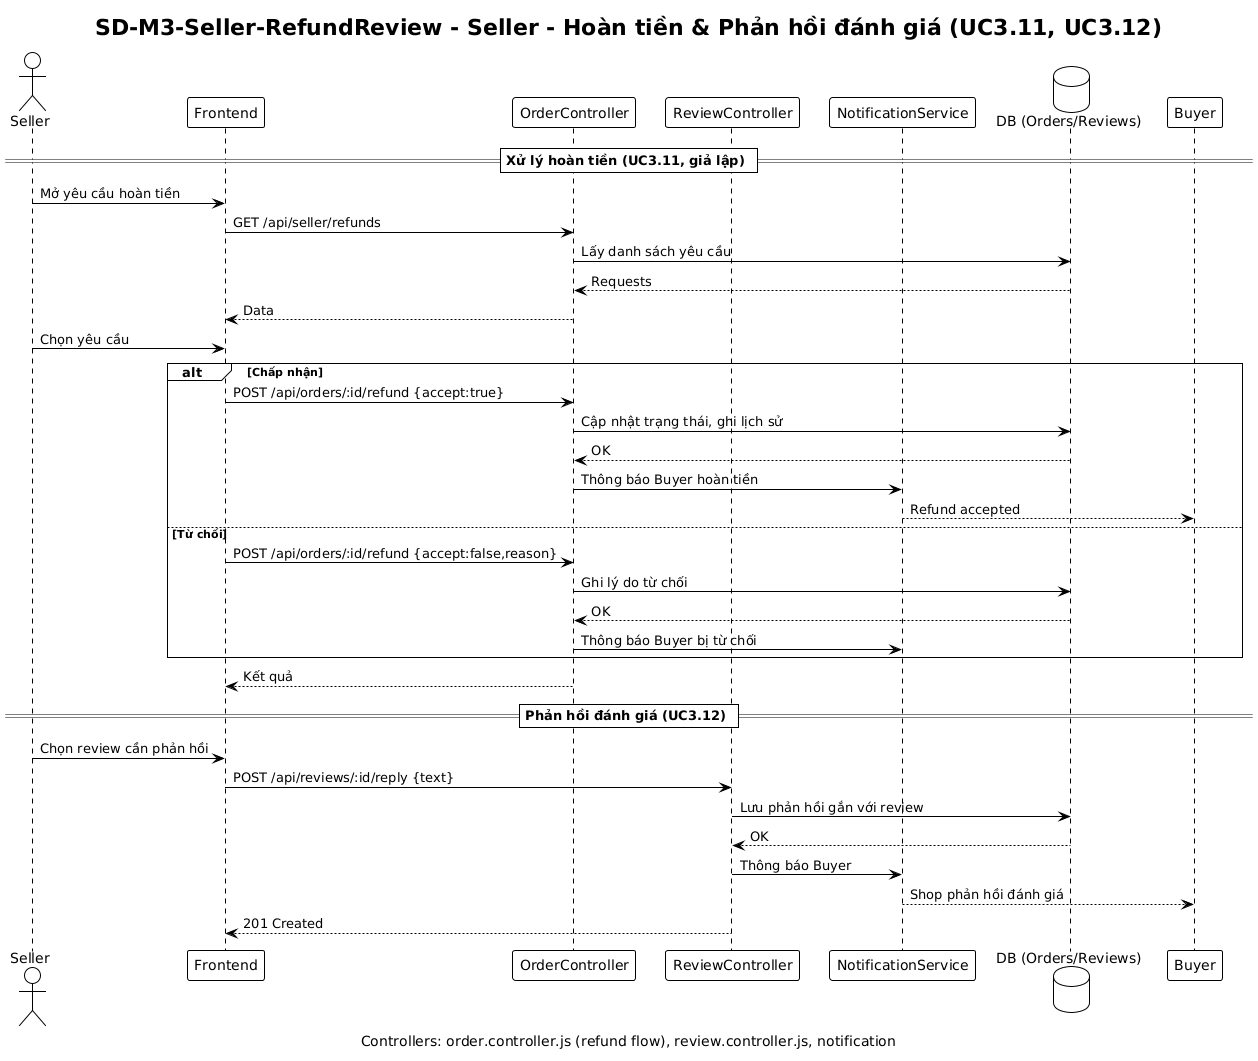
\includegraphics[width=\textwidth]{Images/Sequence diagrams/SD-M3-Seller-RefundReview.png}
  \caption{Sequence Diagram - Hoàn tiền và Phản hồi Đánh giá của Seller (SD-M3-Seller-RefundReview)}
\end{figure}

\subsection{Module 4 – Hệ thống Quản trị}

Module này mô tả luồng tương tác trong công cụ quản trị: quản lý tài khoản, quản lý nội dung, xử lý báo cáo vi phạm, và thống kê phân tích. Các diagram thể hiện cách Frontend giao tiếp với Admin Controllers (UsersController, PostsController, ProductsController, ReportsController, DashboardController) và Database.

\subsubsection{SD-M4-Admin-AccountsContent}

Diagram này mô tả chuỗi tương tác trong quá trình quản lý tài khoản và nội dung của Admin.

\textbf{UC4.1 – Quản lý tài khoản:} Admin Frontend gửi GET \texttt{/api/admin/users?filters=...} đến admin API với tham số lọc và admin JWT. AdminController xác thực token và vai trò Admin, truy vấn DB, trả về danh sách người dùng. Để thực hiện hành động: Frontend gửi PATCH \texttt{/api/admin/users/:id/toggle-active} hoặc PATCH \texttt{/api/admin/users/:id/role}. Controller xác thực quyền, cập nhật trong DB, trả về 200.

\textbf{UC4.2 – Quản lý nội dung:} Admin Frontend gửi GET \texttt{/api/admin/posts} hoặc \texttt{/api/admin/products} kèm admin JWT. AdminController xác thực token và vai trò Admin, truy vấn DB, trả về danh sách. Để xóa: Frontend gửi DELETE \texttt{/api/admin/posts/:id} hoặc \texttt{/api/admin/products/:id}. Controller xác thực quyền, xóa nội dung trong DB và trả về 200.

\begin{figure}[H]
  \centering
  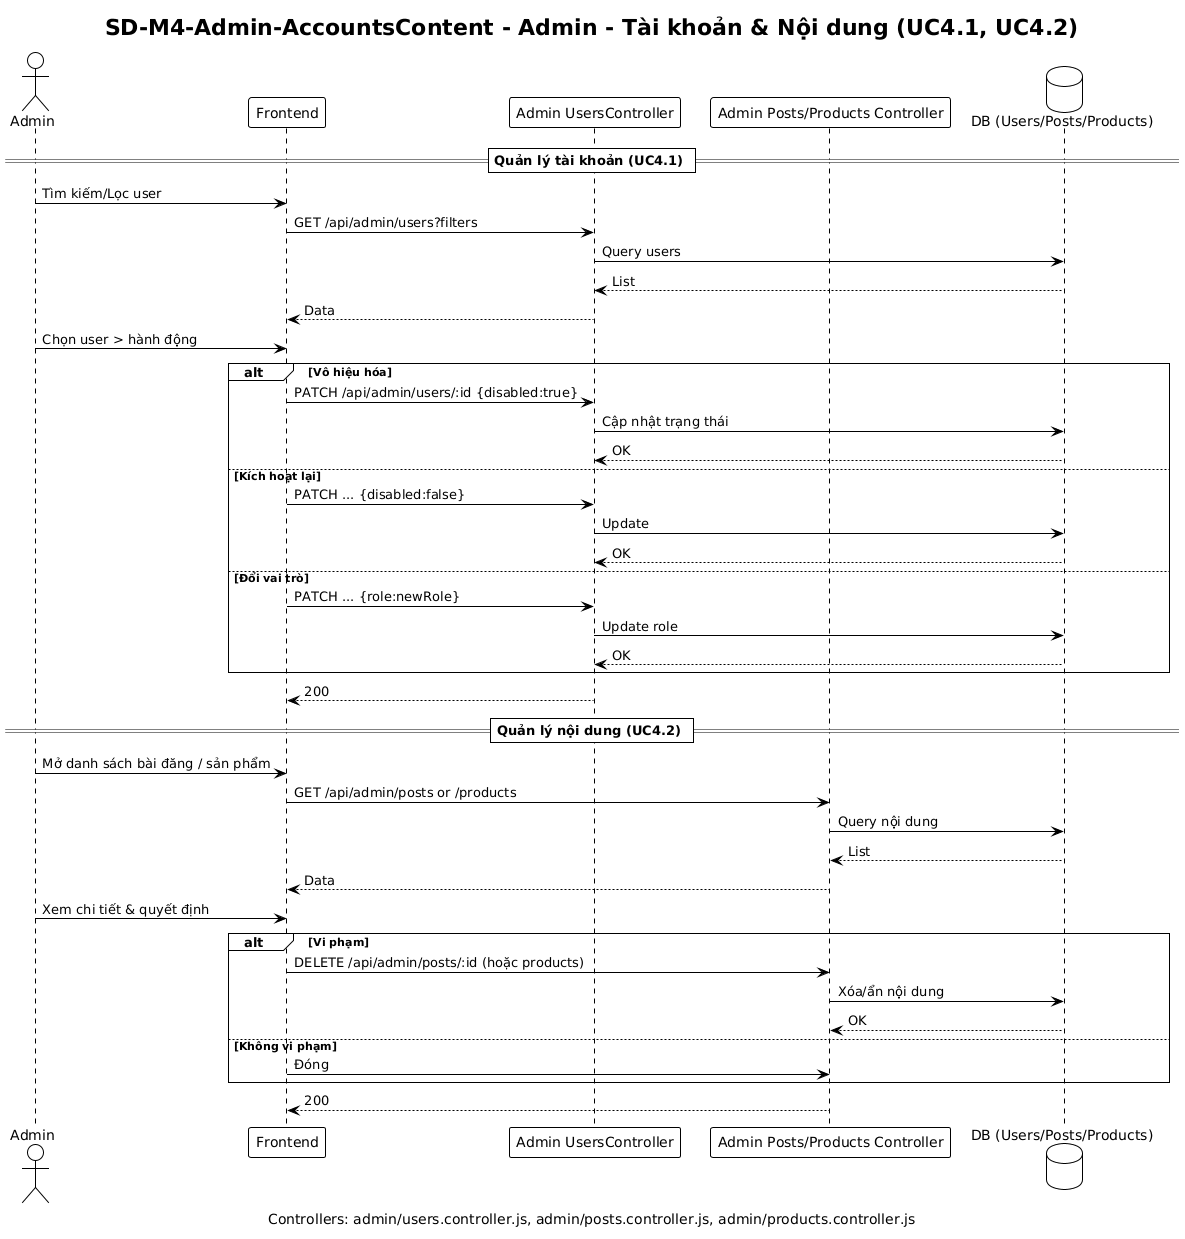
\includegraphics[width=\textwidth]{Images/Sequence diagrams/SD-M4-Admin-AccountsContent.png}
  \caption{Sequence Diagram - Quản lý Tài khoản và Nội dung của Admin (SD-M4-Admin-AccountsContent)}
\end{figure}

\subsubsection{SD-M4-Admin-ReportsAnalytics}

Diagram này mô tả chuỗi tương tác trong quá trình xử lý báo cáo và xem thống kê của Admin.

\textbf{UC4.3 – Xử lý báo cáo vi phạm:} Admin Frontend gửi GET \texttt{/api/reports?status=pending} đến admin API kèm admin JWT. ReportController xác thực, truy vấn DB lấy danh sách báo cáo pending, trả về danh sách. Để xem chi tiết: Frontend gửi GET \texttt{/api/reports/:reportId}. Để xử lý: Frontend gửi PATCH \texttt{/api/reports/:reportId/resolve} kèm action và admin JWT. Controller xác thực quyền, thực thi hành động trong DB, trả về 200.

\textbf{UC4.4 – Thống kê và phân tích:} Admin Frontend gửi GET \texttt{/api/admin/dashboard} hoặc \texttt{/api/admin/dashboard/growth?days=...} kèm admin JWT. AdminController xác thực, truy vấn DB tổng hợp số liệu về người dùng, bài đăng, sản phẩm, đơn hàng, doanh thu và growth, trả về dữ liệu thống kê.

\begin{figure}[H]
  \centering
  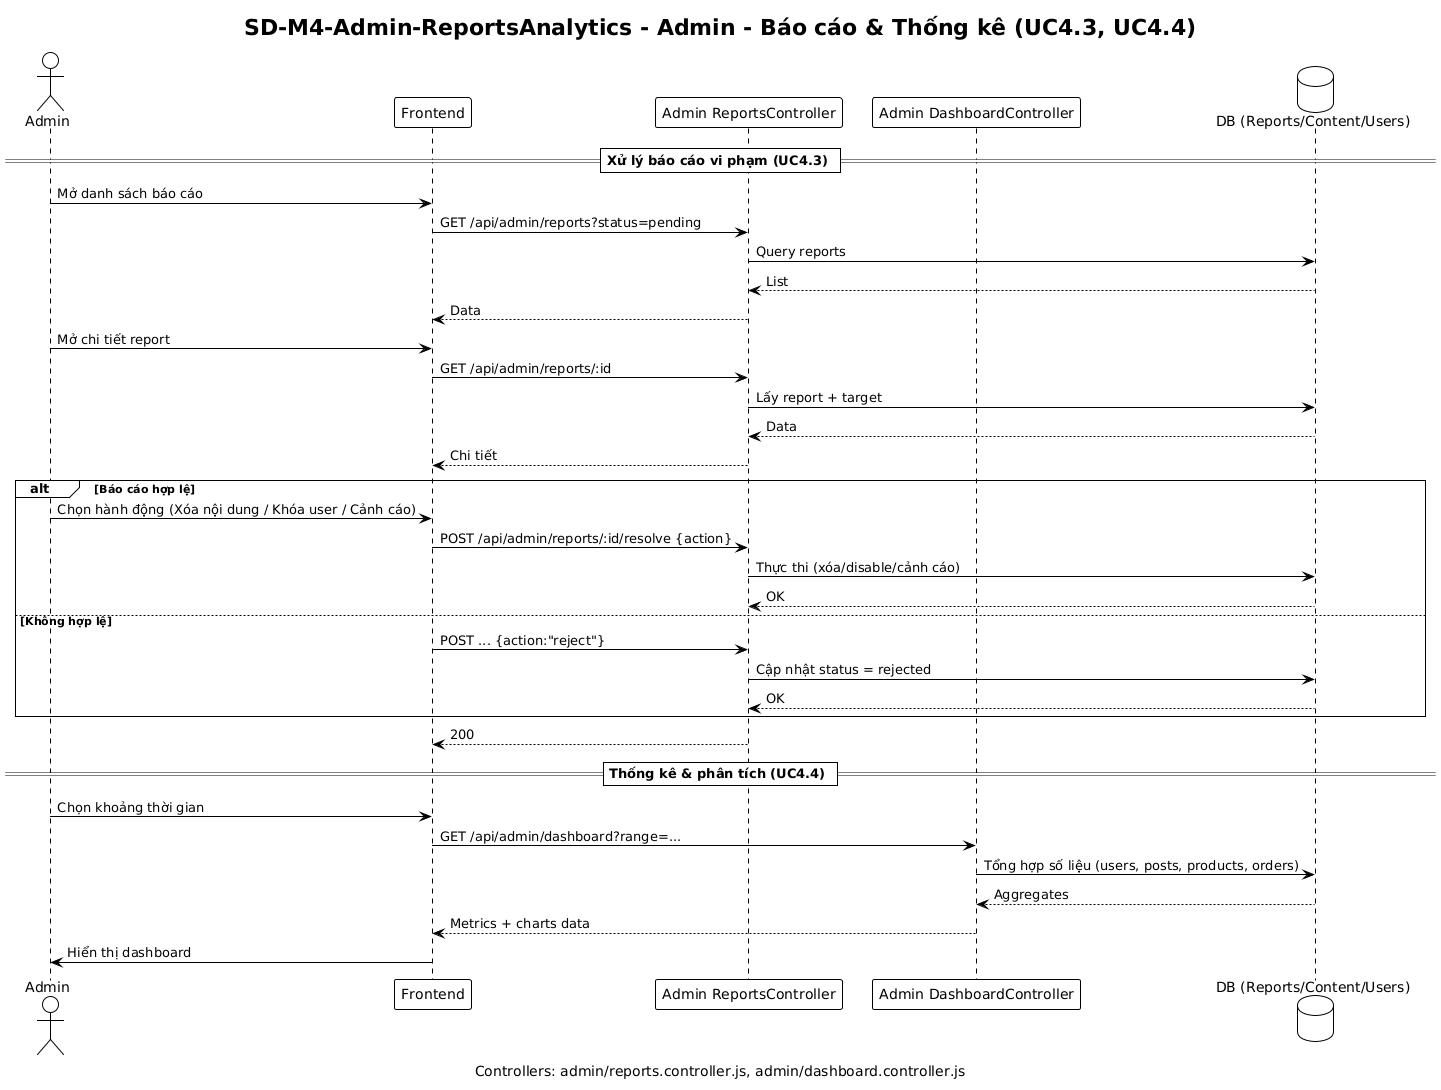
\includegraphics[width=\textwidth]{Images/Sequence diagrams/SD-M4-Admin-ReportsAnalytics.png}
  \caption{Sequence Diagram - Báo cáo và Thống kê của Admin (SD-M4-Admin-ReportsAnalytics)}
\end{figure}

\subsection{Module 5 – Tích hợp AI hỗ trợ}

Module này mô tả luồng tương tác trong tính năng AI hỗ trợ tạo nội dung và AI Shopping Assistant: generate text, generate image+text, quản lý lịch sử nội dung AI và chatbox tư vấn mua sắm. Các diagram thể hiện cách Frontend giao tiếp với AIController, AI Assistant Controller, AI Service, external AI providers và Database.

\subsubsection{SD-M5-AIContentCreation}

Diagram này mô tả chuỗi tương tác trong quá trình tạo nội dung sử dụng AI và tư vấn mua sắm qua chatbox.

\textbf{UC5.1 – Generate Text:} Frontend gửi POST \texttt{/api/ai/generate-text} kèm mô tả, ý tưởng, hình ảnh (nếu có) và JWT token. AIController xác thực, gọi AI Service. AI Service chuẩn hóa đầu vào, gọi text provider để sinh nội dung dạng cấu trúc, sau đó chạy bước đánh giá chất lượng (\textit{evaluate + score}). Nếu điểm chưa đạt ngưỡng, AI Service tự động \textit{refine prompt} và \textit{regenerate} theo vòng lặp giới hạn số lần thử. Nếu provider chính gặp lỗi quota/rate-limit, hệ thống retry/backoff và có thể chuyển sang provider dự phòng. Khi nội dung đạt ngưỡng, hệ thống lưu lịch sử và trả về văn bản với trạng thái chất lượng phù hợp.

\textbf{UC5.2 – Generate Image + Text:} Frontend gửi POST \texttt{/api/ai/generate-image-text} kèm mô tả, ý tưởng, hình ảnh đầu vào (nếu có) và JWT token. AIController xác thực và gọi AI Service. AI Service thực thi đầy đủ pipeline UC5.1 để bảo đảm chất lượng phần chữ, sau đó chuẩn hóa prompt ảnh (ưu tiên tiếng Anh) và gọi chuỗi image provider theo thứ tự chính/phụ. Nếu provider chính thất bại, hệ thống tự fallback sang provider kế tiếp. Nếu gặp lỗi quota/rate-limit hoặc toàn bộ provider ảnh không khả dụng, hệ thống \textit{degrade gracefully}: vẫn trả phần chữ đã đạt chuẩn cùng trạng thái lỗi ảnh để người dùng tiếp tục thao tác.

\textbf{UC5.3 – AI Shopping Assistant Chatbox:} Frontend gửi POST \texttt{/api/ai-assistant/chat} kèm câu hỏi, lịch sử hội thoại gần nhất, bộ nhớ phiên và JWT token. AiAssistantController xác thực người dùng, chuẩn hóa lịch sử, sau đó gọi AiAssistantService. Service phân tích intent, truy vấn dữ liệu sản phẩm/đơn hàng thuộc quyền truy cập của người dùng, gọi AI text provider để tạo phản hồi và trả về \texttt{reply}, \texttt{followUps}, \texttt{memory}, \texttt{cards} và \texttt{quickActions}. Frontend hiển thị phản hồi trong chatbox và thực hiện quick action như mở sản phẩm, thêm vào giỏ hàng hoặc xem chi tiết đơn hàng.

\begin{figure}[H]
  \centering
  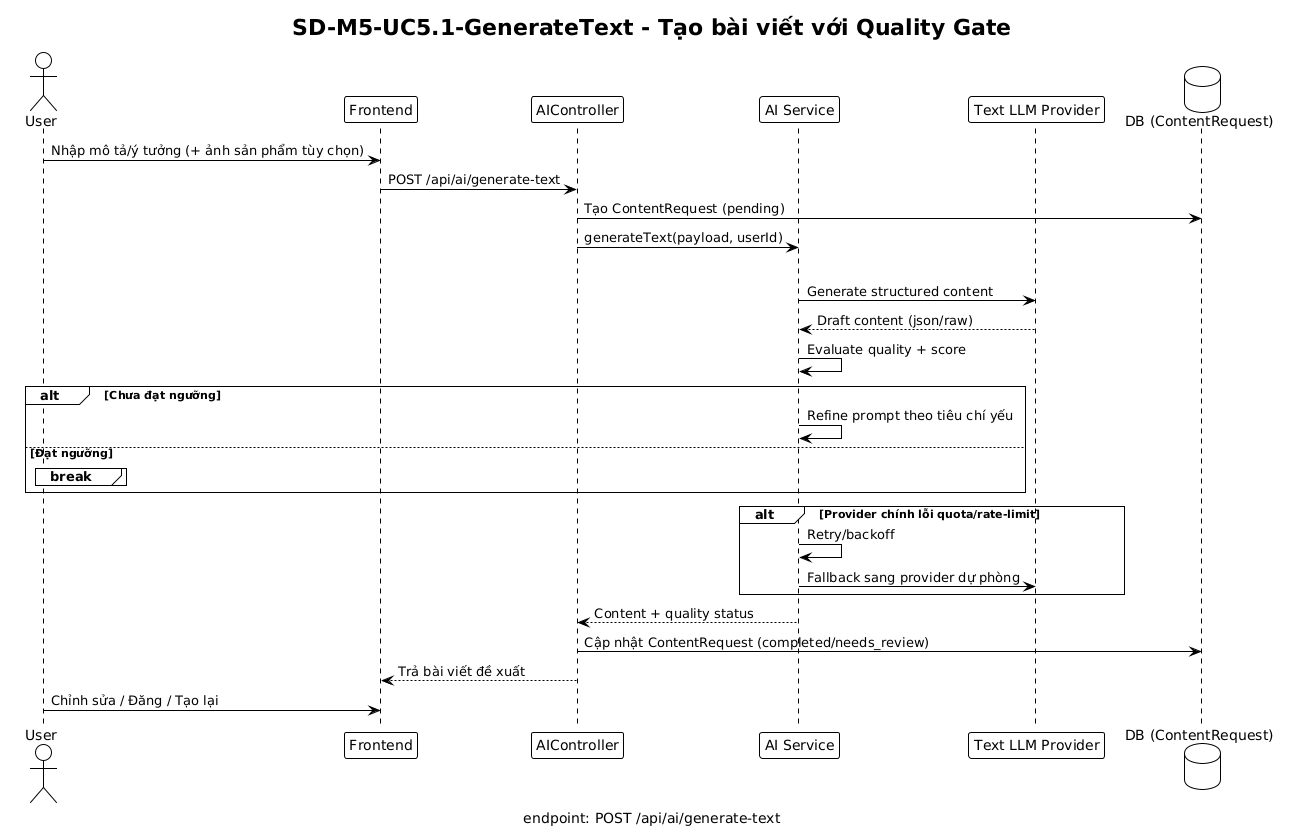
\includegraphics[width=\textwidth]{Images/Sequence diagrams/SD-M5-UC5.1-GenerateText.png}
  \caption{Sequence Diagram - Tạo bài viết với AI (SD-M5-UC5.1-GenerateText)}
\end{figure}

\begin{figure}[H]
  \centering
  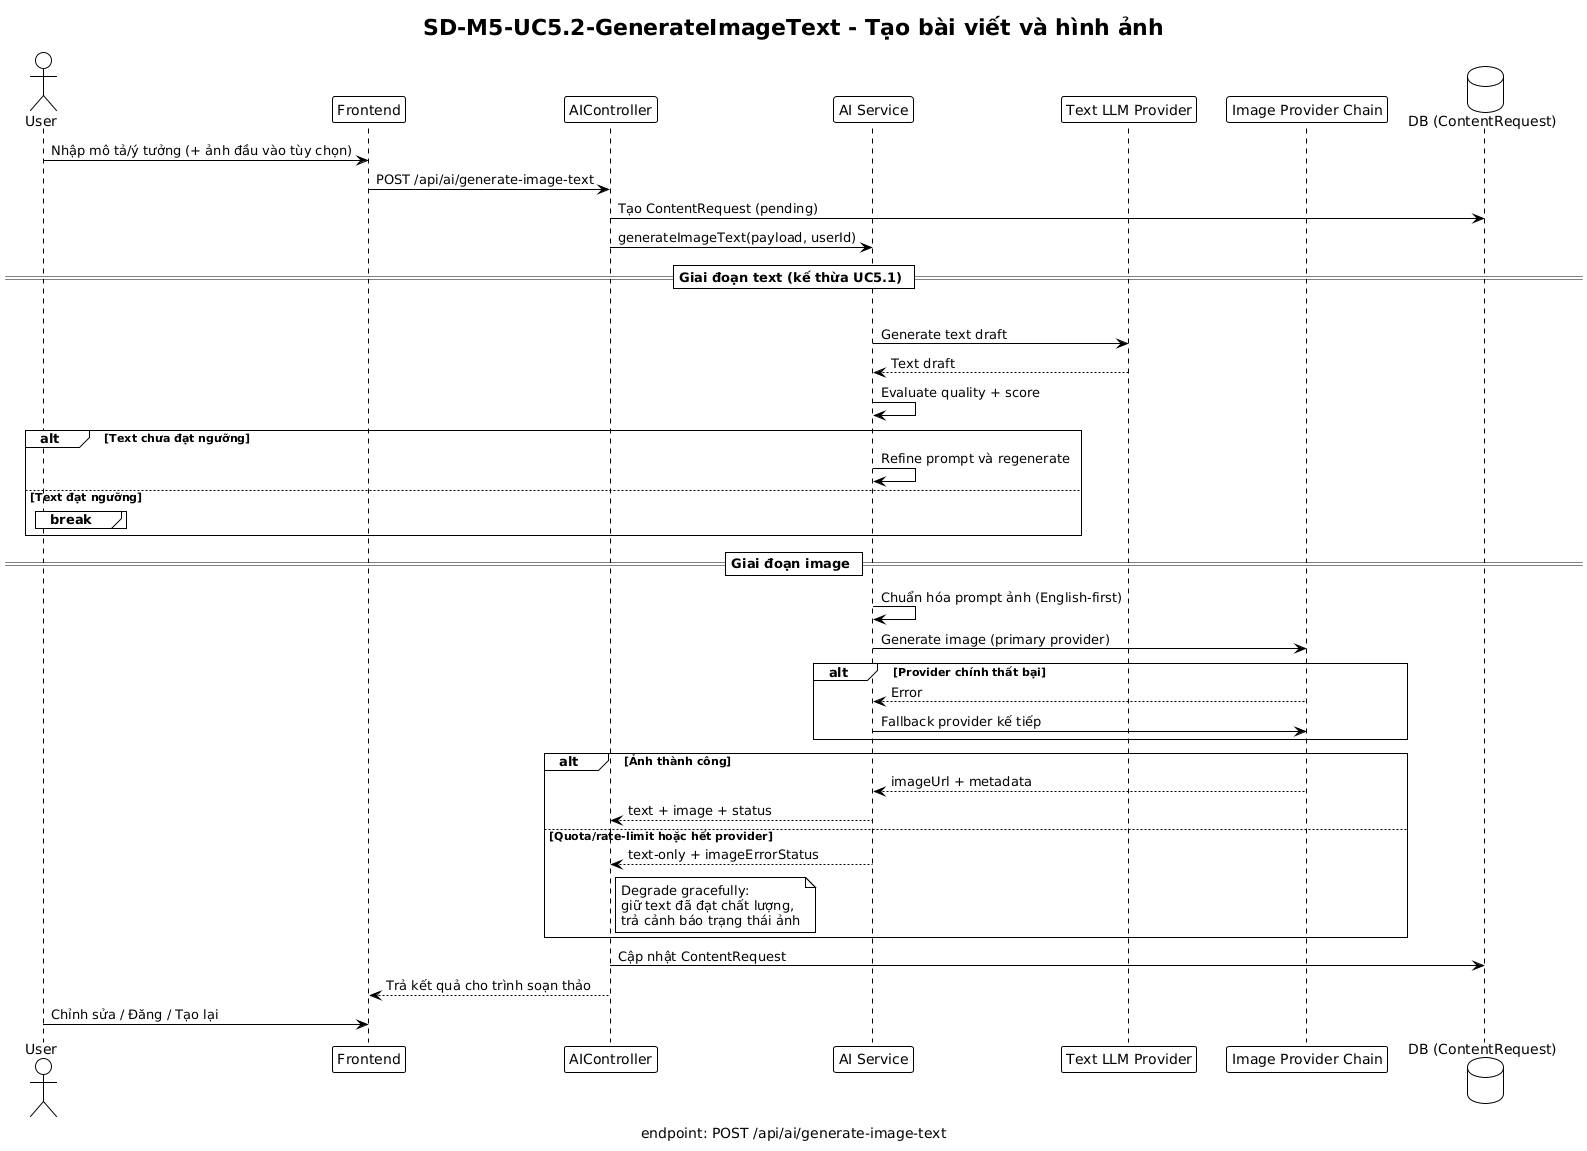
\includegraphics[width=\textwidth]{Images/Sequence diagrams/SD-M5-UC5.2-GenerateImageText.png}
  \caption{Sequence Diagram - Tạo bài viết và hình ảnh với AI (SD-M5-UC5.2-GenerateImageText)}
\end{figure}

\begin{figure}[H]
  \centering
  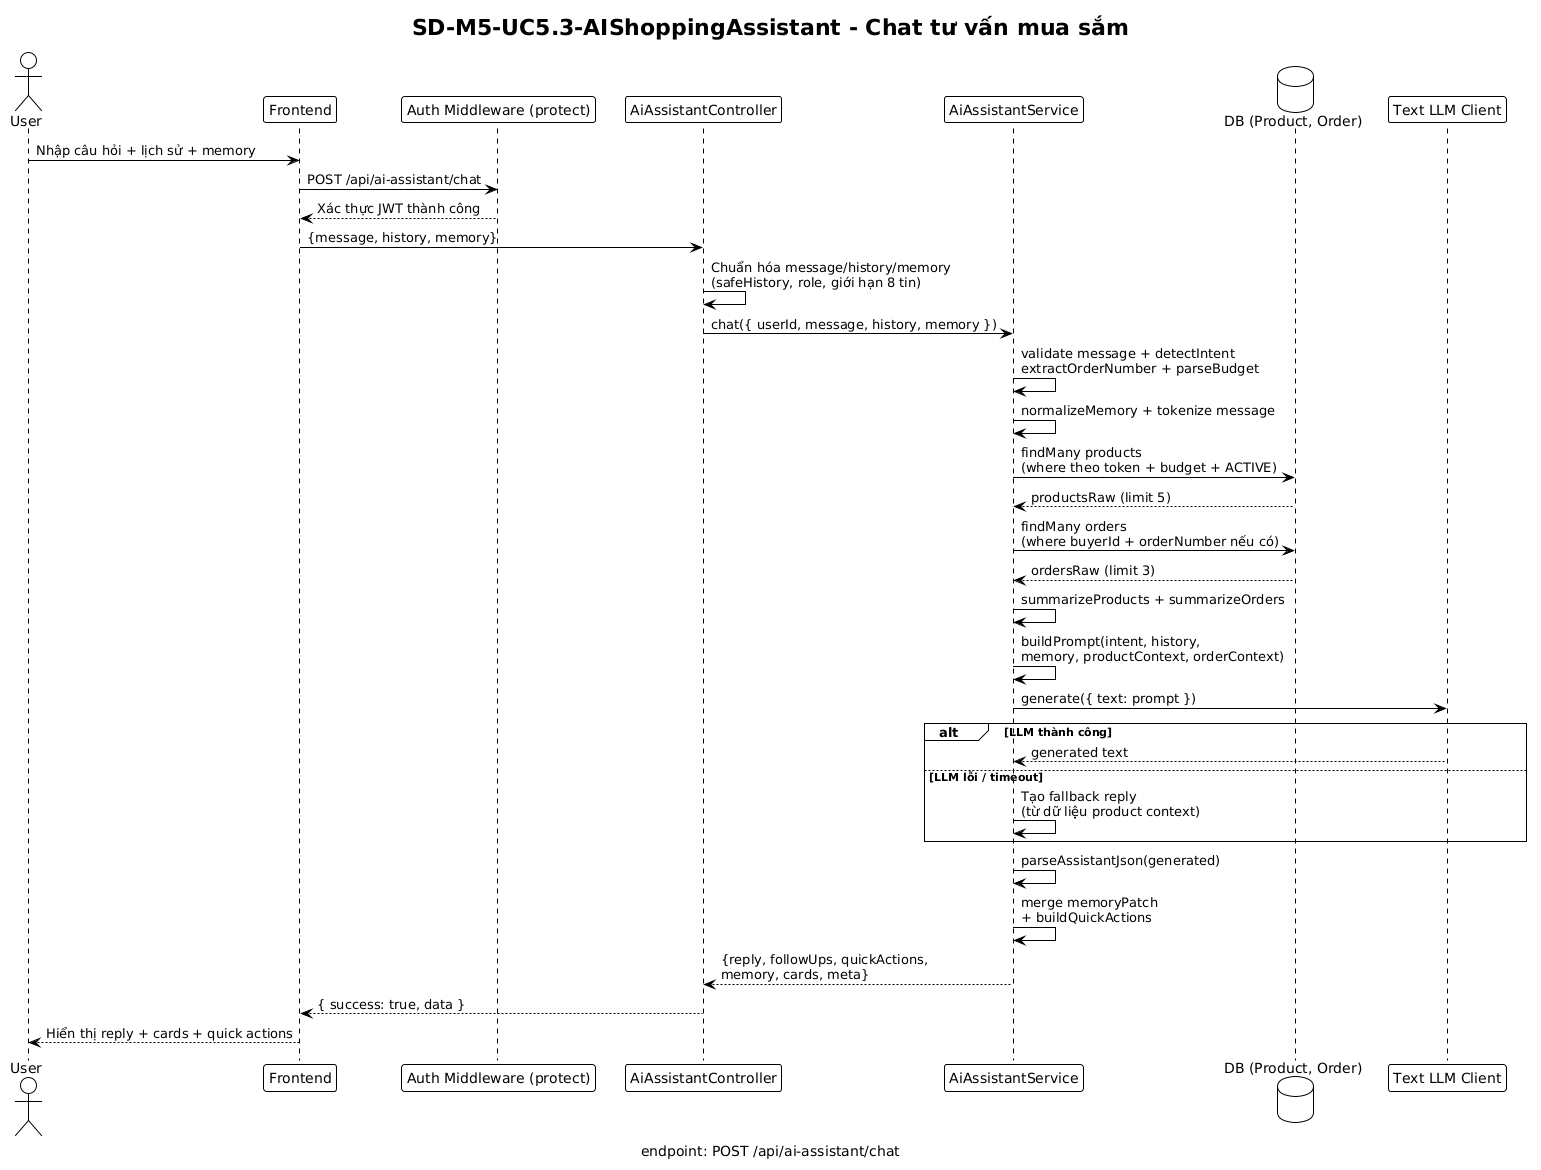
\includegraphics[width=\textwidth]{Images/Sequence diagrams/SD-M5-UC5.3-AIShoppingAssistant.png}
  \caption{Sequence Diagram - AI Shopping Assistant Chatbox (SD-M5-UC5.3-AIShoppingAssistant)}
\end{figure}

\subsection{Module 6 – Lên lịch và Điều phối Bài đăng}

Module này mô tả luồng tương tác trong tính năng lên lịch đăng bài: tạo lịch đăng, quản lý bài đăng đã lên lịch, và tự động xuất bản qua cron job. Các diagram thể hiện cách Frontend giao tiếp với PostController, Database và CronScheduler.

\subsubsection{SD-M6-PostScheduling}

Diagram này mô tả chuỗi tương tác trong quá trình lên lịch đăng bài và quản lý bài đăng đã lên lịch, bao gồm cả tác vụ tự động của cron job.

\textbf{UC6.1 – Lên lịch đăng bài:} Frontend gửi POST \texttt{/api/scheduled-posts} kèm nội dung, thời gian xuất bản (scheduledTime) và JWT token. ScheduledPostController xác thực, kiểm tra thời gian trong tương lai, lưu bài đăng với trạng thái \textit{scheduled} vào DB, trả về 201.

\textbf{UC6.2 – Quản lý bài đăng đã lên lịch:} Frontend gửi GET \texttt{/api/scheduled-posts} kèm JWT token. ScheduledPostController xác thực, truy vấn DB lấy danh sách bài đăng \textit{scheduled}, trả về danh sách. Để chỉnh sửa: Frontend gửi PUT \texttt{/api/scheduled-posts/:id}. Để đăng ngay: Frontend gửi POST \texttt{/api/scheduled-posts/:id/publish}. Để xóa: Frontend gửi DELETE \texttt{/api/scheduled-posts/:id}. Controller xử lý trong DB, trả về kết quả.

\textbf{Cron Job – Xuất bản tự động:} CronScheduler chạy định kỳ, truy vấn DB lấy scheduled posts có trạng thái \textit{scheduled} và thời gian đã đến. Scheduler tạo bản ghi Post tương ứng, cập nhật scheduled post thành \textit{published} và lưu publishedPostId.

\begin{figure}[H]
  \centering
  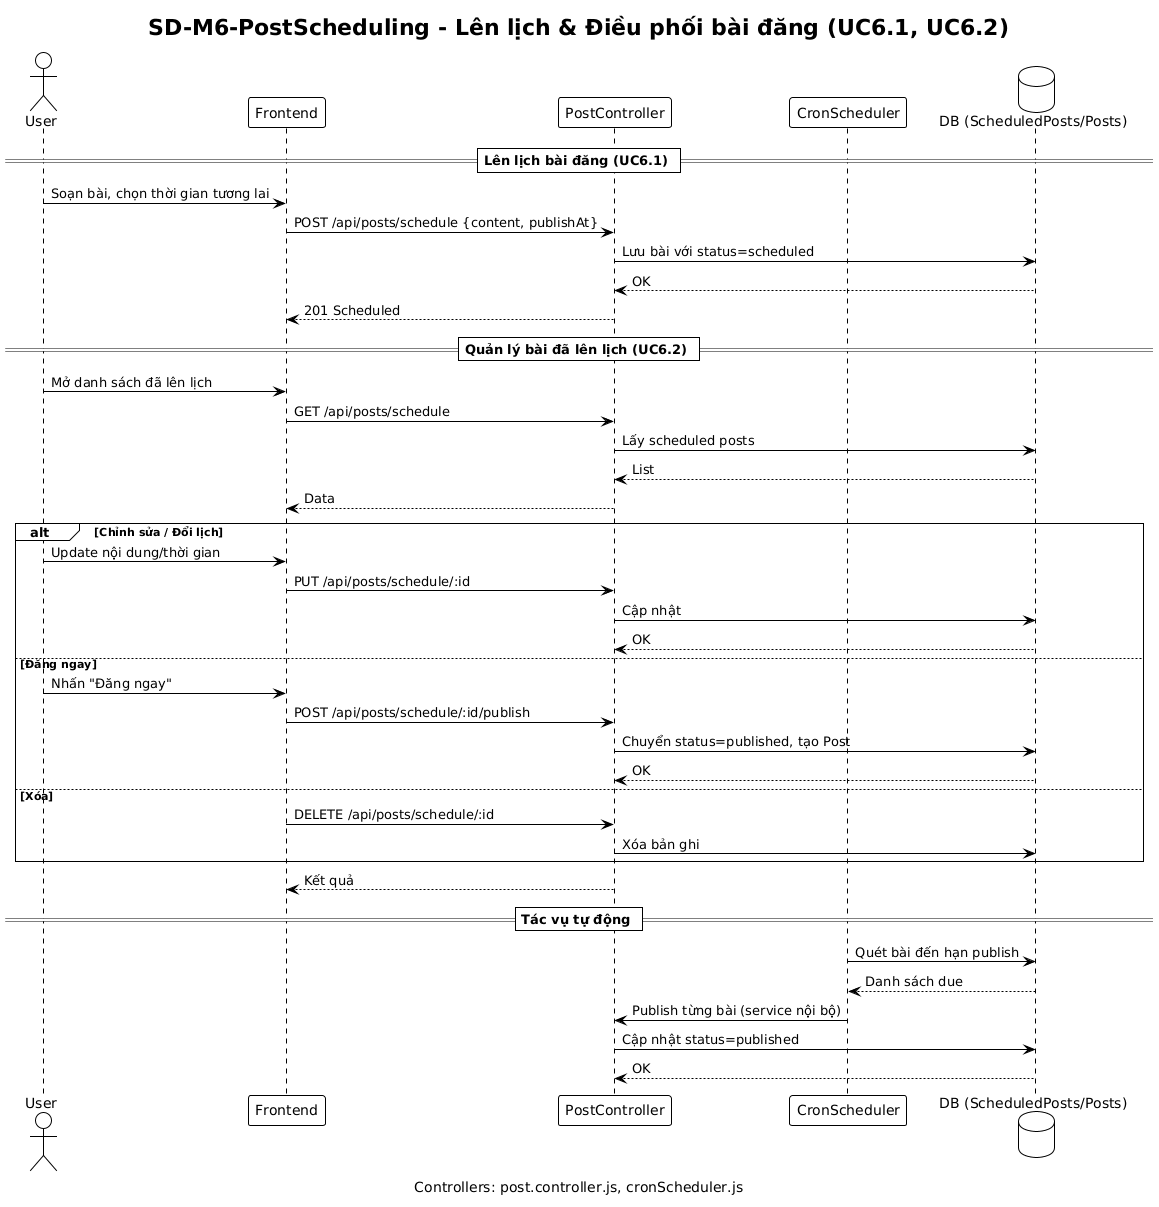
\includegraphics[width=\textwidth]{Images/Sequence diagrams/SD-M6-PostScheduling.png}
  \caption{Sequence Diagram - Lên lịch và Điều phối Bài đăng (SD-M6-PostScheduling)}
\end{figure}

\subsection{Module 7 – Hệ thống Thông báo}

Module này mô tả luồng tương tác trong hệ thống thông báo: tạo và gửi thông báo (tương tác xã hội, giao dịch), quản lý thông báo (xem, đánh dấu đã đọc, xóa), và cấu hình nhận thông báo. Các diagram thể hiện cách Frontend giao tiếp với NotificationController, NotificationService (Socket) và Database.

\subsubsection{SD-M7-NotificationSystem}

Diagram này mô tả chuỗi tương tác trong toàn bộ hệ thống thông báo, bao gồm bốn use case chính.

\textbf{UC7.1 – Thông báo tương tác:} Khi có sự kiện like, comment hoặc follow, service nghiệp vụ gọi NotificationService để tạo thông báo. NotificationService kiểm tra preference của người nhận, lưu thông báo vào DB và emit qua Socket.IO nếu người nhận online. Thông báo vẫn được lưu để hiển thị khi người nhận mở lại ứng dụng.

\textbf{UC7.2 – Thông báo giao dịch:} Khi có sự kiện giao dịch, hệ thống gọi NotificationController tạo thông báo. Controller lưu vào DB và gửi qua Socket đến Buyer/Seller. Nếu người nhận online và bật nhận, họ nhận real-time qua WebSocket.

\textbf{UC7.3 – Quản lý thông báo:} Frontend gửi GET \texttt{/api/notifications} kèm JWT token. NotificationController xác thực, truy vấn DB lấy danh sách thông báo (sắp xếp theo thời gian, mới nhất trước), trả về danh sách. Để đánh dấu đã đọc: Frontend gửi PATCH \texttt{/api/notifications/:id} với \texttt{\{read: true\}}. Để xóa: Frontend gửi DELETE \texttt{/api/notifications/:id}. Controller cập nhật/xóa trong DB, trả về 200.

\textbf{UC7.4 – Cài đặt thông báo:} Frontend gửi GET \texttt{/api/notifications/preferences} kèm JWT token. NotificationController xác thực, đọc cấu hình hiện tại từ privacySettings của user và trả về cấu hình. Để cập nhật: Frontend gửi PATCH \texttt{/api/notifications/preferences} kèm cấu hình mới và JWT token. Controller xác thực, lưu cấu hình vào DB, trả về 200. Cấu hình được áp dụng ngay lập tức.

\begin{figure}[H]
  \centering
  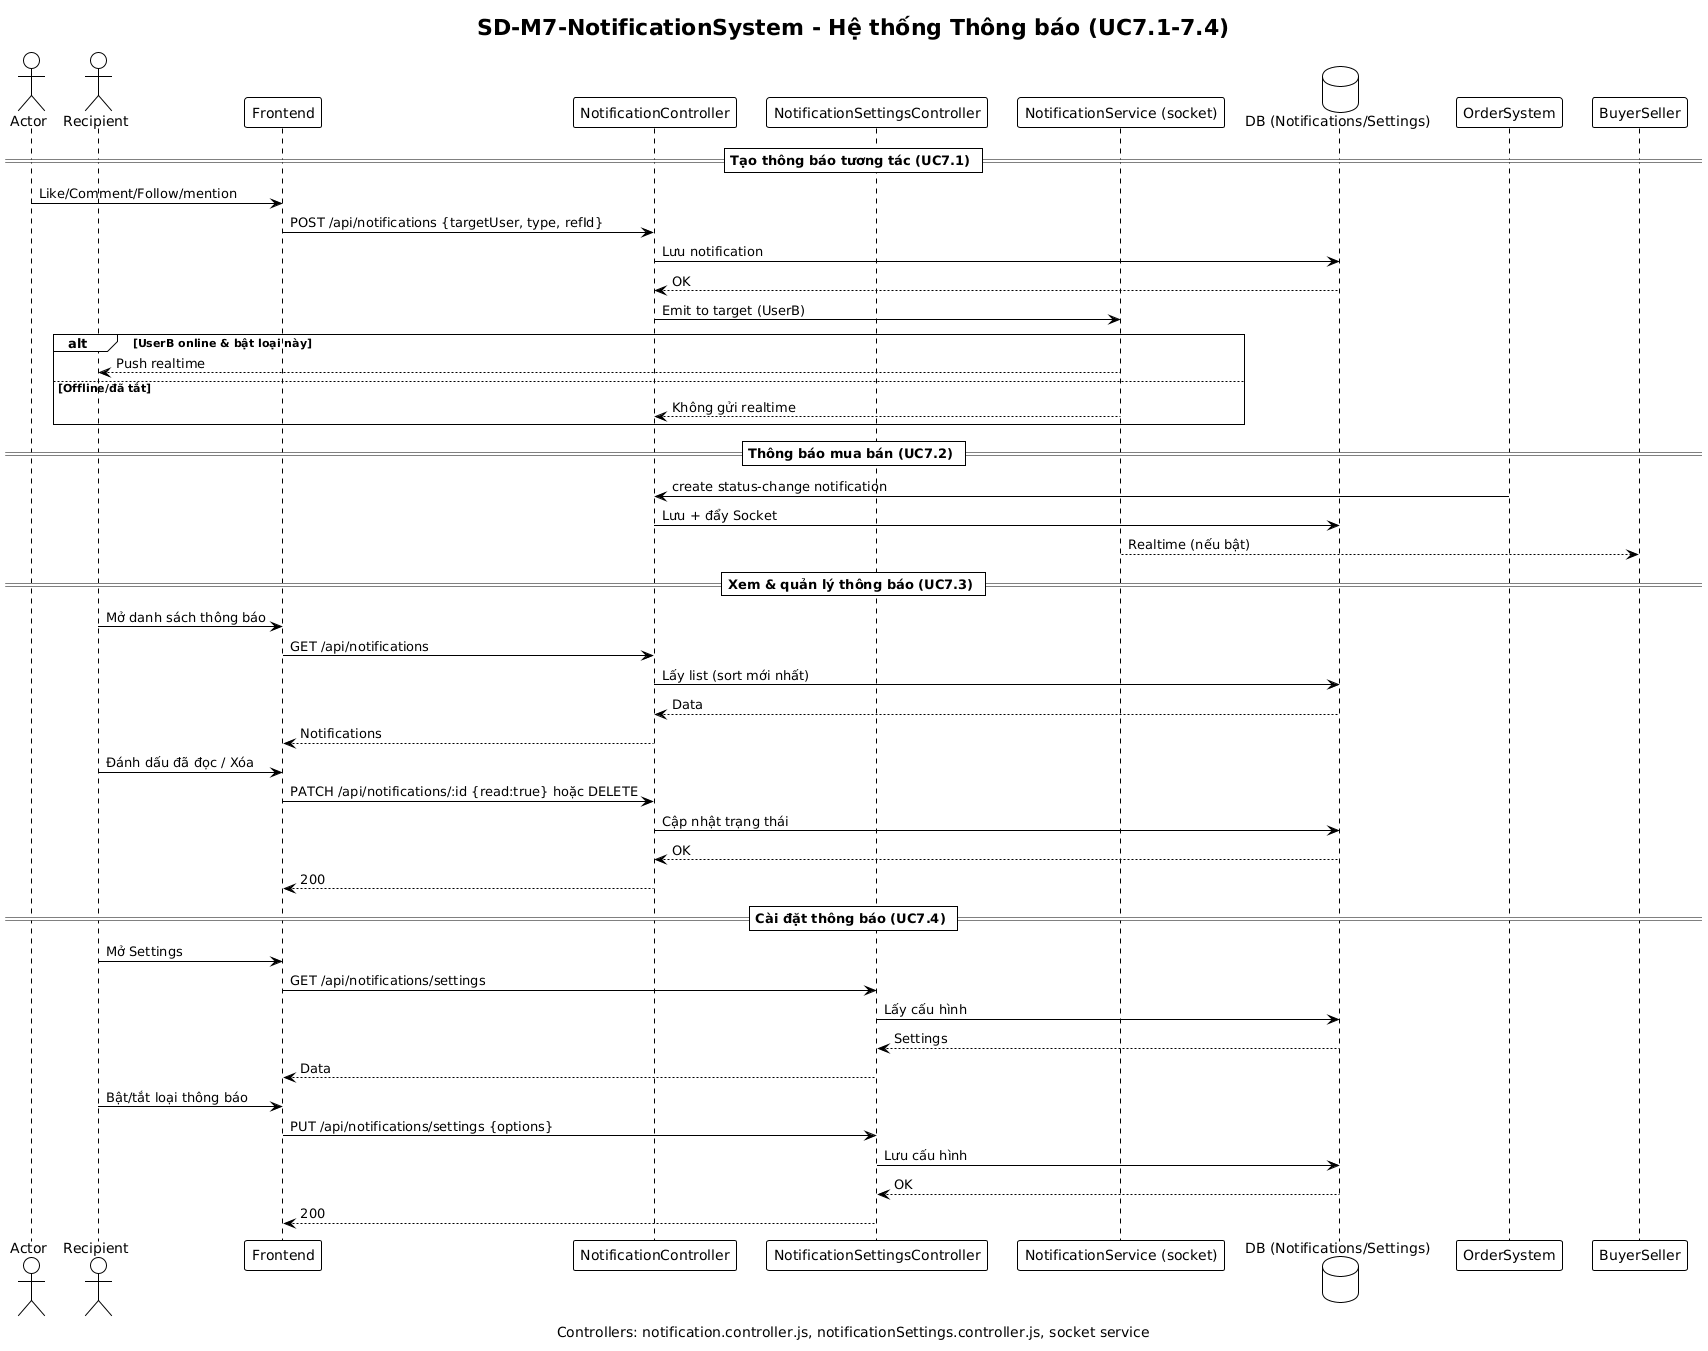
\includegraphics[width=\textwidth]{Images/Sequence diagrams/SD-M7-NotificationSystem.png}
  \caption{Sequence Diagram - Hệ thống Thông báo (SD-M7-NotificationSystem)}
\end{figure}
